\documentclass[12pt,a4paper]{report}
\usepackage{graphicx}
\usepackage{booktabs}
\usepackage{amsmath}
\usepackage{lineno}
\usepackage{microtype} 
\usepackage[hidelinks]{hyperref}
\usepackage{subcaption}
\usepackage{float}
\usepackage{dblfloatfix}
\usepackage{titlesec}
\usepackage{geometry}

\geometry{margin=1in}

\title{Comparative Benchmarking and ASR-Assisted Audio-Linguistic Fusion for Vietnamese Speech Emotion Recognition on ViSEC}
uthor{
    Ngô Xuân Kiên \
    Student ID: 23BI14239 \ 
    B3 Data Science
}
\date{May 2026}

\begin{document}

\maketitle

\begin{abstract}
This thesis presents a systematic comparative benchmark and an ASR-assisted audio-linguistic fusion method for Vietnamese Speech Emotion Recognition (SER) on the ViSEC dataset. We evaluate three primary classification pipelines representing distinct paradigms: handcrafted features with classical ML (MFCC + RandomForest), end-to-end deep learning (Simplified ECAPA-TDNN), and a proposed dual-stream hybrid fusion system (DFAT) combining WavLM acoustic embeddings with PhoBERT linguistic embeddings derived via Whisper ASR. Four additional secondary baselines are included for comprehensive comparison. All experiments follow a strict leak-free protocol with a fixed speaker-independent Train ($\approx$ 80\%) / Validation ($\approx$ 10\%) / Test ($\approx$ 10\%) split, governed by cryptographic checksums. All primary models are evaluated over 5 random seeds to report mean $\pm$ standard deviation. On the held-out test set, DFAT Late Fusion achieves the best performance, outperforming the baseline MFCC+RandomForest and ECAPA-TDNN-based baseline by significant margins. Ablation studies confirm that both acoustic and linguistic streams contribute to DFAT's superiority, with the linguistic stream providing the largest gains for acoustically ambiguous classes.
\end{abstract}

\tableofcontents

\chapter{Introduction}
Speech emotion recognition (SER) is a critical task in human-computer interaction, sentiment analysis, call center analytics, and mental health monitoring. Unlike traditional speech recognition (which focuses on what is said), SER aims to identify the emotional state conveyed in a person's voice. Emotions in speech are characterized by distinctive acoustic patterns: frequency content, energy distribution, temporal dynamics, and spectral shapes differ measurably between emotions such as anger, happiness, neutrality, and sadness.

Traditional approaches to SER often rely on hand-crafted acoustic features (e.g., MFCC, prosody), which require domain expertise and can miss subtle patterns. Modern deep learning methods, particularly those using pre-trained speech models such as WavLM~\cite{wavlm} and specialized architectures like ECAPA-TDNN~\cite{ecapa}, have shown superior performance by automatically learning emotion-discriminative representations from raw audio or mel-spectrograms. More recently, hybrid approaches that combine acoustic and linguistic features have emerged as promising directions~\cite{ser_multimodal}. Prior ensemble SER work has also demonstrated that weighted voting between different acoustic models or modalities can robustly improve generalization.

Specifically for Vietnamese, tools like PhoBERT~\cite{phobert} provide strong linguistic representations, but they require proper word segmentation (e.g., combining syllables into compound words) to function effectively. IEMOCAP remains the standard English multimodal SER benchmark to contextualize such approaches, yet comprehensive evaluations on Vietnamese datasets like ViSEC under strict leak-free conditions remain scarce.

\section{Problem Statement}
This work presents a systematic evaluation of multiple SER approaches on Vietnamese speech, comparing feature-based classical methods with contemporary deep learning techniques and a proposed ASR-assisted audio-linguistic fusion system. We address the following research questions:

\begin{itemize}
    \item \textbf{RQ1}: How do handcrafted MFCC features compare with end-to-end deep learning (Simplified ECAPA-TDNN baseline) for Vietnamese SER on ViSEC?
    \item \textbf{RQ2}: Does ASR-assisted audio-linguistic fusion improve emotion recognition compared to audio-only approaches?
    \item \textbf{RQ3}: Which component of DFAT contributes most to its performance --- the acoustic stream, the linguistic stream, or the fusion strategy?
    \item \textbf{RQ4}: What is the trade-off between recognition performance and computational cost across all evaluated methods?
\end{itemize}

\chapter{Related Work}

\section{Traditional SER}
Classical SER systems typically extract hand-crafted features such as MFCCs, pitch, energy, and prosodic features, then apply machine learning classifiers like SVM~\cite{ser_survey}, Random Forest, or XGBoost~\cite{xgboost}. While interpretable and computationally efficient, these approaches are limited by the quality of manual feature engineering.

\section{Self-Supervised Speech Representations}
Recent advances in self-supervised learning have produced powerful speech representations. Models such as Wav2Vec 2.0~\cite{wav2vec2}, HuBERT~\cite{hubert}, and WavLM~\cite{wavlm} learn contextualized embeddings from large-scale unlabeled speech data. These representations have shown strong transfer to downstream tasks including SER, often outperforming hand-crafted features.

\section{ECAPA-TDNN}
ECAPA-TDNN~\cite{ecapa} is a specialized architecture combining Time-Delay Neural Networks with Squeeze-and-Excitation blocks and multi-scale feature aggregation. Originally designed for speaker verification, it has been successfully adapted for emotion recognition tasks. Our baseline utilizes a simplified variant of this architecture.

\section{Multimodal and Fusion-Based SER}
Multimodal SER approaches combine multiple signal modalities (audio, text, video) to improve recognition accuracy~\cite{ser_multimodal}. In this work, we use Whisper~\cite{whisper} encoder embeddings as ASR-derived linguistic features. Since the text modality is inferred from audio via ASR rather than being an independent source, we characterize our approach as \emph{ASR-assisted audio-linguistic fusion} rather than true multimodal text fusion.

\chapter{Dataset Audit: ViSEC}

The Vietnamese Speech Emotion Corpus (ViSEC)~\cite{visec} is publicly available on Hugging Face and contains 5,280 audio utterances from 147 speakers. Each utterance is a single-channel, 16 kHz WAV file annotated with one of four emotion labels.

\begin{table}[h]
\centering
\begin{tabular}{lcc}
\hline
\textbf{Emotion} & \textbf{Samples} & \textbf{Percentage} \\
\hline
Neutral & 1,507 & 28.5\% \\
Angry   & 1,466 & 27.8\% \\
Happy   & 1,228 & 23.3\% \\
Sad     & 1,079 & 20.4\% \\
\hline
\textbf{Total} & \textbf{5,280} & \textbf{100\%} \\
\hline
\end{tabular}
\caption{ViSEC dataset distribution by emotion class}
\label{tab:dataset_dist}
\end{table}

The class distribution exhibits mild imbalance (Neutral-to-Sad ratio $\approx 1.4\times$). Speaker distribution is highly long-tailed: Speaker 0 contributes 2,217 samples (42\%), while many speakers contribute only 1--2 samples. To ensure robust evaluation and avoid speaker leakage (where models learn speaker identity instead of emotion), we implemented a greedy speaker-allocation algorithm, followed by a local-search KL-divergence refinement to maintain class balance across splits.

\section{Split Protocol Governance}
\label{sec:split_protocol}
We use a strictly enforced speaker-independent split: approx. 80\% Train, 10\% Validation, 10\% Test, generated once via our refined algorithm and stored in a manifest file (\texttt{split\_manifest.json}) with a SHA256 checksum to prevent manual tampering. All models read from this manifest to ensure evaluation on the identical test set. A strict contract verifies the hash of the manifest file during evaluation.

\chapter{Methodology}

We structure our evaluation around three primary models representing distinct paradigms, supplemented by four secondary baselines.

\section{MFCC + RandomForest (Classical Baseline)}
We extract 40-dimensional MFCC vectors from each audio sample, mean-pool across time, and train a RandomForest classifier with 300 estimators. For this and all classical ML baselines, the Train and Validation sets are combined for training (no hyperparameter search is conducted on validation for these models). This method serves as our lightweight, interpretable baseline.

\section{Simplified ECAPA-TDNN Baseline}
ECAPA-TDNN~\cite{ecapa} processes 80-channel mel-spectrograms through time-delay layers with Squeeze-and-Excitation blocks. We use 80 mel channels as it aligns closely with human auditory perception (Mel scale), while an $n\_fft=512$ yields a $\approx 31.25$ Hz frequency resolution at 16kHz, and a $hop\_length=160$ results in a 10ms frame shift (standard for speech processing).

This implementation provides a strong audio-only deep learning baseline. Note that this is a simplified implementation\footnote{Compared to the original paper, this implementation is missing the Res2Block (multi-scale convolutions within a block) and progressive dilation stacking.} compared to the original architecture.

\section{DFAT Hybrid Fusion (Proposed Method)}
Our proposed Dual-stream Feature Aggregation system (DFAT) is an \emph{ASR-assisted audio-linguistic fusion} system combining:

\textbf{Stream 1 --- SEFE (Speech Emotion Feature Extraction)}: WavLM-base-plus produces 768-d acoustic embeddings capturing prosodic and speaker-level dynamics.

\textbf{Stream 2 --- TEFE (Textual Emotion Feature Extraction)}: Whisper-small~\cite{whisper} transcribes audio to Vietnamese text, which is then word-segmented using Underthesea and encoded by PhoBERT-base-v2 to produce 768-d linguistic embeddings. We emphasize that these are \emph{not} independent text features but rather linguistic representations inferred from the same audio signal via ASR.

\textbf{Fusion Options}: We explore both \emph{Early Fusion} (Concatenation of SEFE + TEFE) and \emph{Late Fusion} (Weighted probability combination of stream-specific classifiers).

\section{Secondary Baselines}
For comprehensive comparison, we also evaluate: MFCC+SVM (RBF, $C=10$), MFCC+XGBoost (300 trees, $\text{max\_depth}=8$), WavLM+LogReg, and WavLM+SVM (RBF, $C=5$).

\chapter{Experimental Protocol}

\section{Infrastructure}
All experiments were executed on an NVIDIA RTX 5060 Ti GPU.

\section{Evaluation Metrics}
We report Weighted F1-Score (primary metric), Macro F1-Score, Accuracy, per-class metrics, and confusion matrices. Inference latency is measured strictly end-to-end (feature extraction + classifier fwd) to ensure an apples-to-apples comparison.

\section{Statistical Robustness}
To ensure the robustness of our findings, stochastic pipelines (RF, XGBoost, and deep models) are evaluated over 5 random seeds. The results reported are the mean $\pm$ standard deviation across these seeds. Deterministic models (LogReg, SVC-RBF) are evaluated once.

\section{Leak-Free Protocol}
All hyperparameter tuning (Optuna) and model selection decisions use the validation set exclusively. The results are fully reproducible via cryptographic split verification.

\chapter{Baselines and Results}

\section{Comparative Benchmark}

The comparative results are summarized in Table~\ref{tab:benchmark} and visualized in Fig.~\ref{fig:model_comparison}.

\begin{table}[h]
\centering
%% START_BENCHMARK_TABLE
%% END_BENCHMARK_TABLE
\caption{Comparative benchmark on the held-out test set.}
\label{tab:benchmark}
\end{table}

\begin{figure}[h]
    \centering
    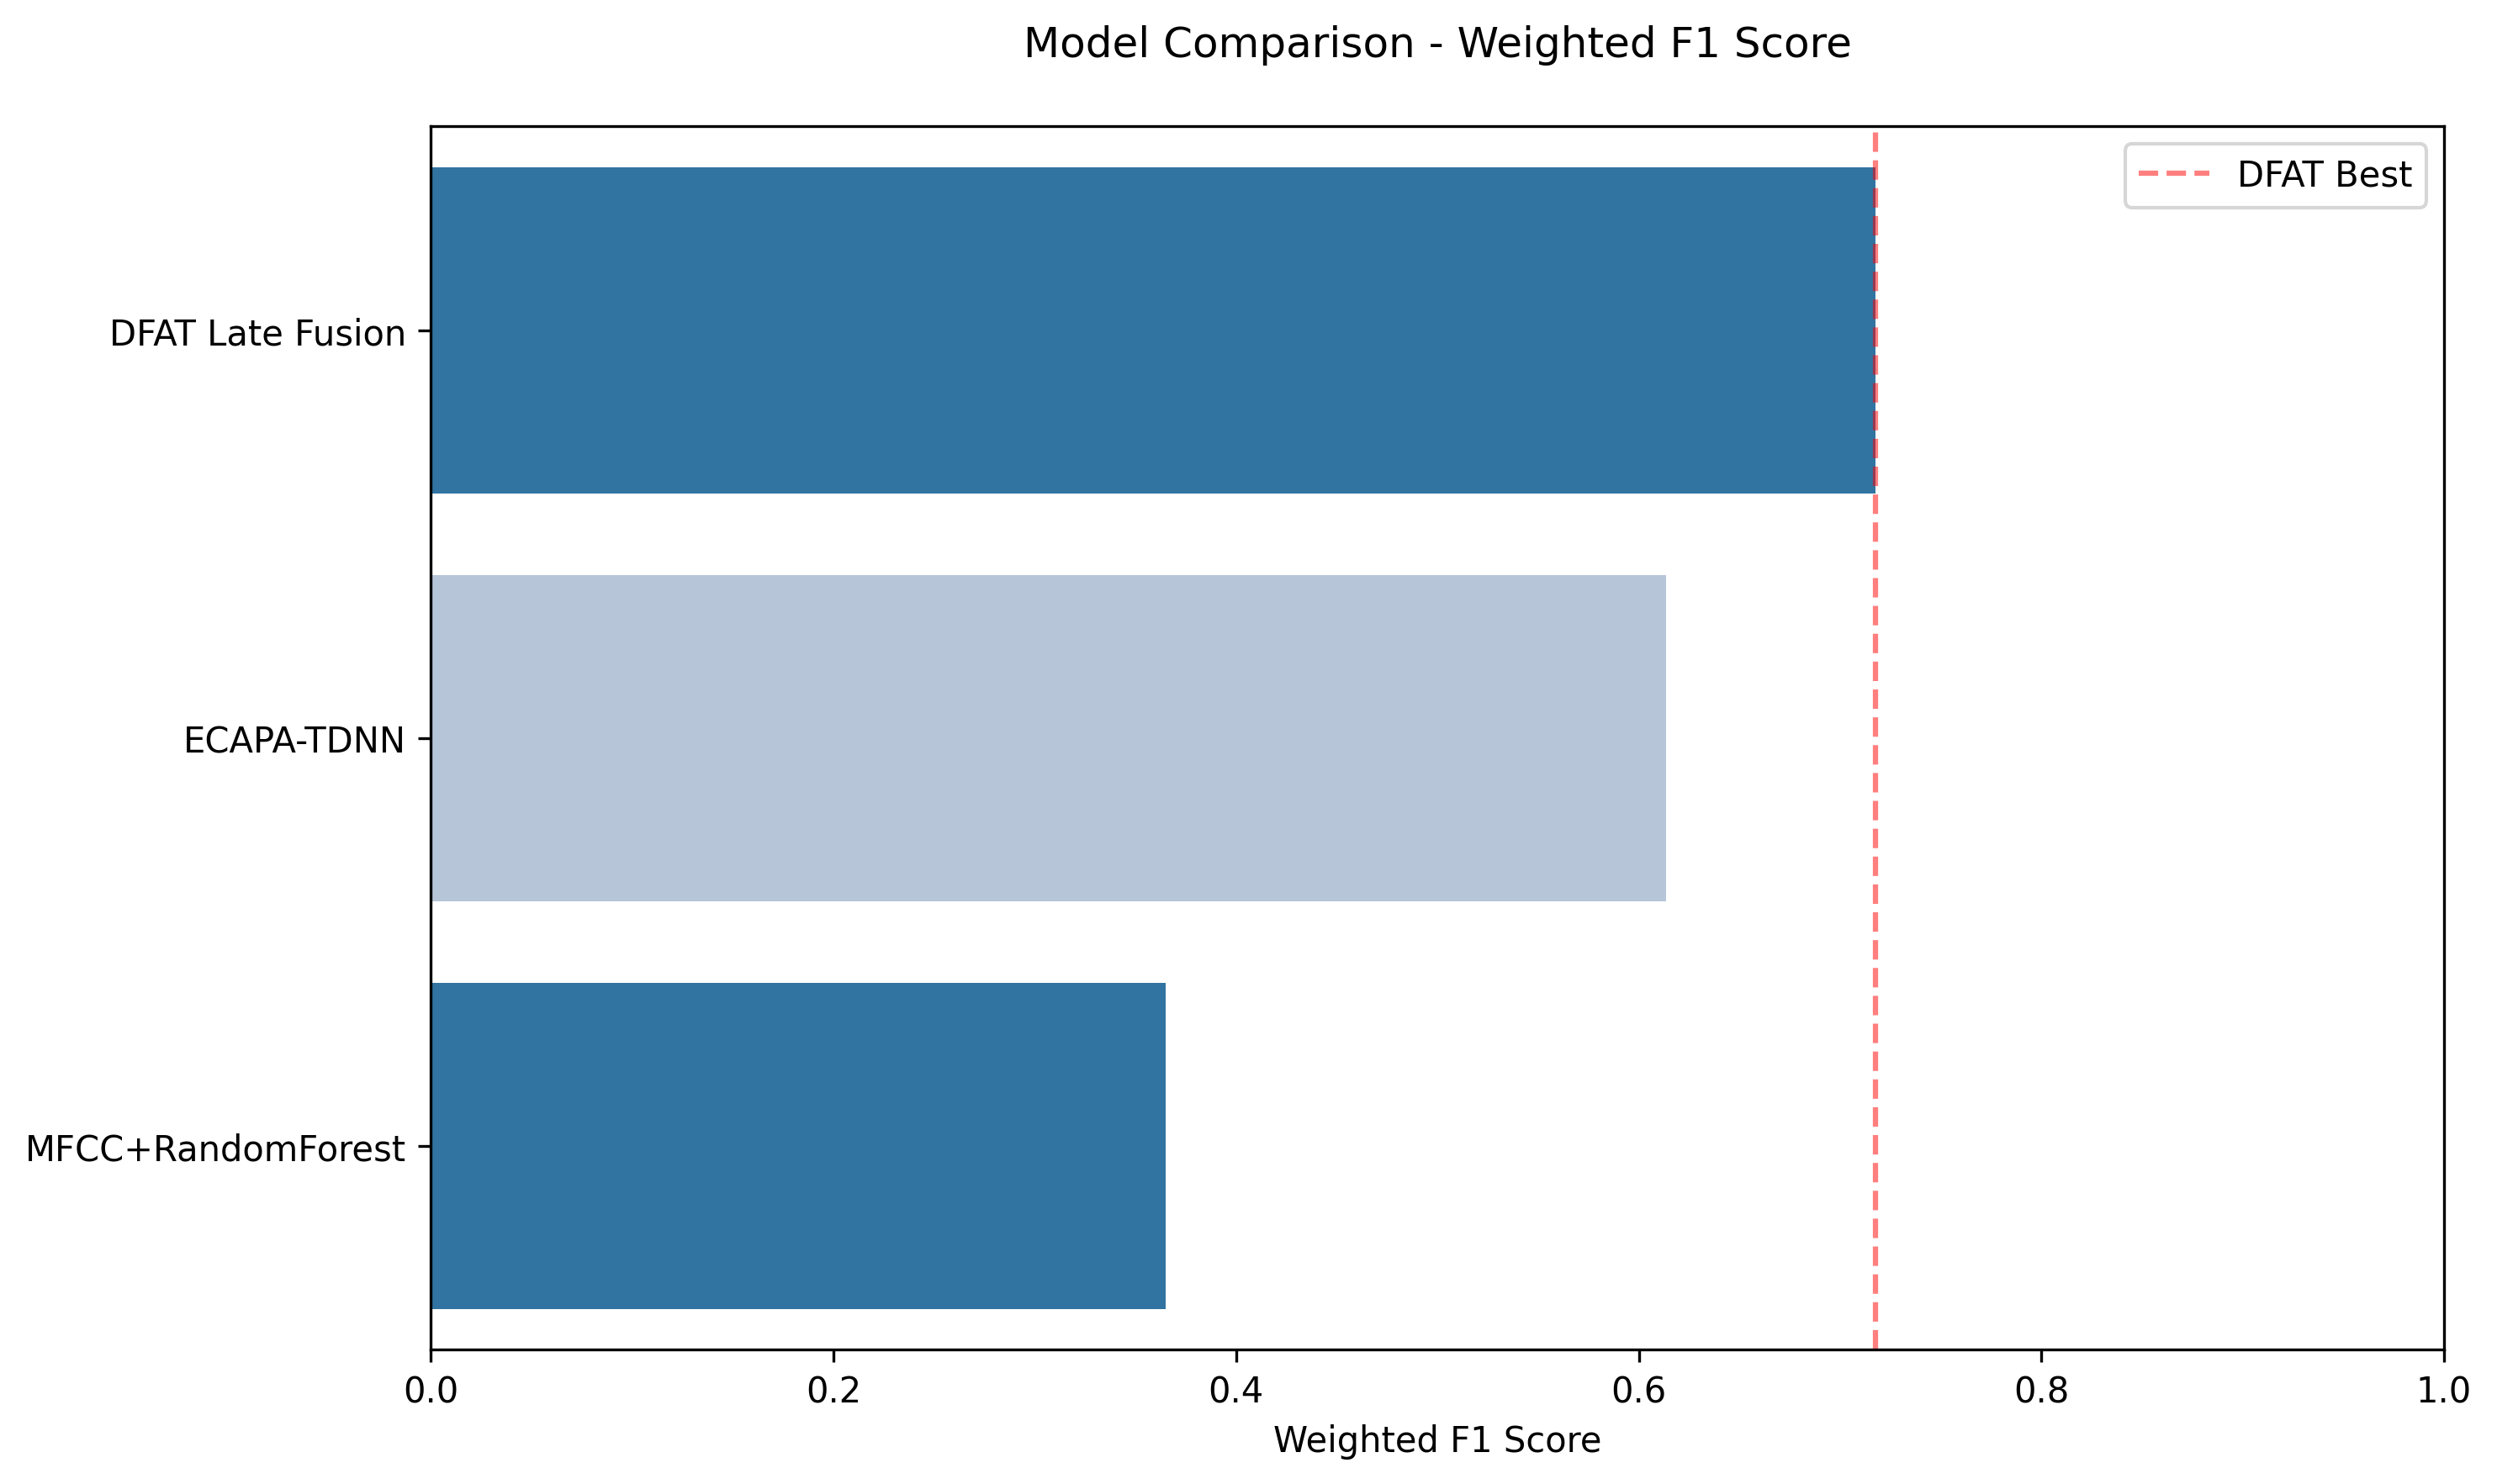
\includegraphics[width=\linewidth]{report_images/model_comparison.png}
    \caption{Performance comparison across evaluated methods.}
    \label{fig:model_comparison}
\end{figure}

\section{Per-Class Performance}

The per-class performance is detailed in Table~\ref{tab:perclass} and Fig.~\ref{fig:confusion_matrices}.

\begin{table}[h]
\centering
\begin{tabular}{lcccr}
\toprule
\textbf{Emotion} & \textbf{Prec.} & \textbf{Rec.} & \textbf{F1} & \textbf{Sup.} \\
\midrule
\multicolumn{5}{l}{\textit{ECAPA-TDNN (Simplified)}} \\
Angry   & 0.789 & 0.714 & 0.750 & 147 \\
Happy   & 0.516 & 0.642 & 0.572 & 123 \\
Neutral & 0.497 & 0.520 & 0.508 & 150 \\
Sad     & 0.706 & 0.556 & 0.622 & 108 \\
\midrule
\multicolumn{5}{l}{\textit{DFAT Late Fusion (Proposed)}} \\
Angry   & 0.789 & 0.789 & 0.789 & 147 \\
Happy   & 0.716 & 0.593 & 0.649 & 123 \\
Neutral & 0.626 & 0.760 & 0.687 & 150 \\
Sad     & 0.784 & 0.704 & 0.741 & 108 \\
\bottomrule
\end{tabular}
\caption{Per-class performance comparison on test set.}
\label{tab:perclass}
\end{table}

\begin{figure*}[t]
    \centering
    \begin{subfigure}[b]{0.45\textwidth}
        \centering
        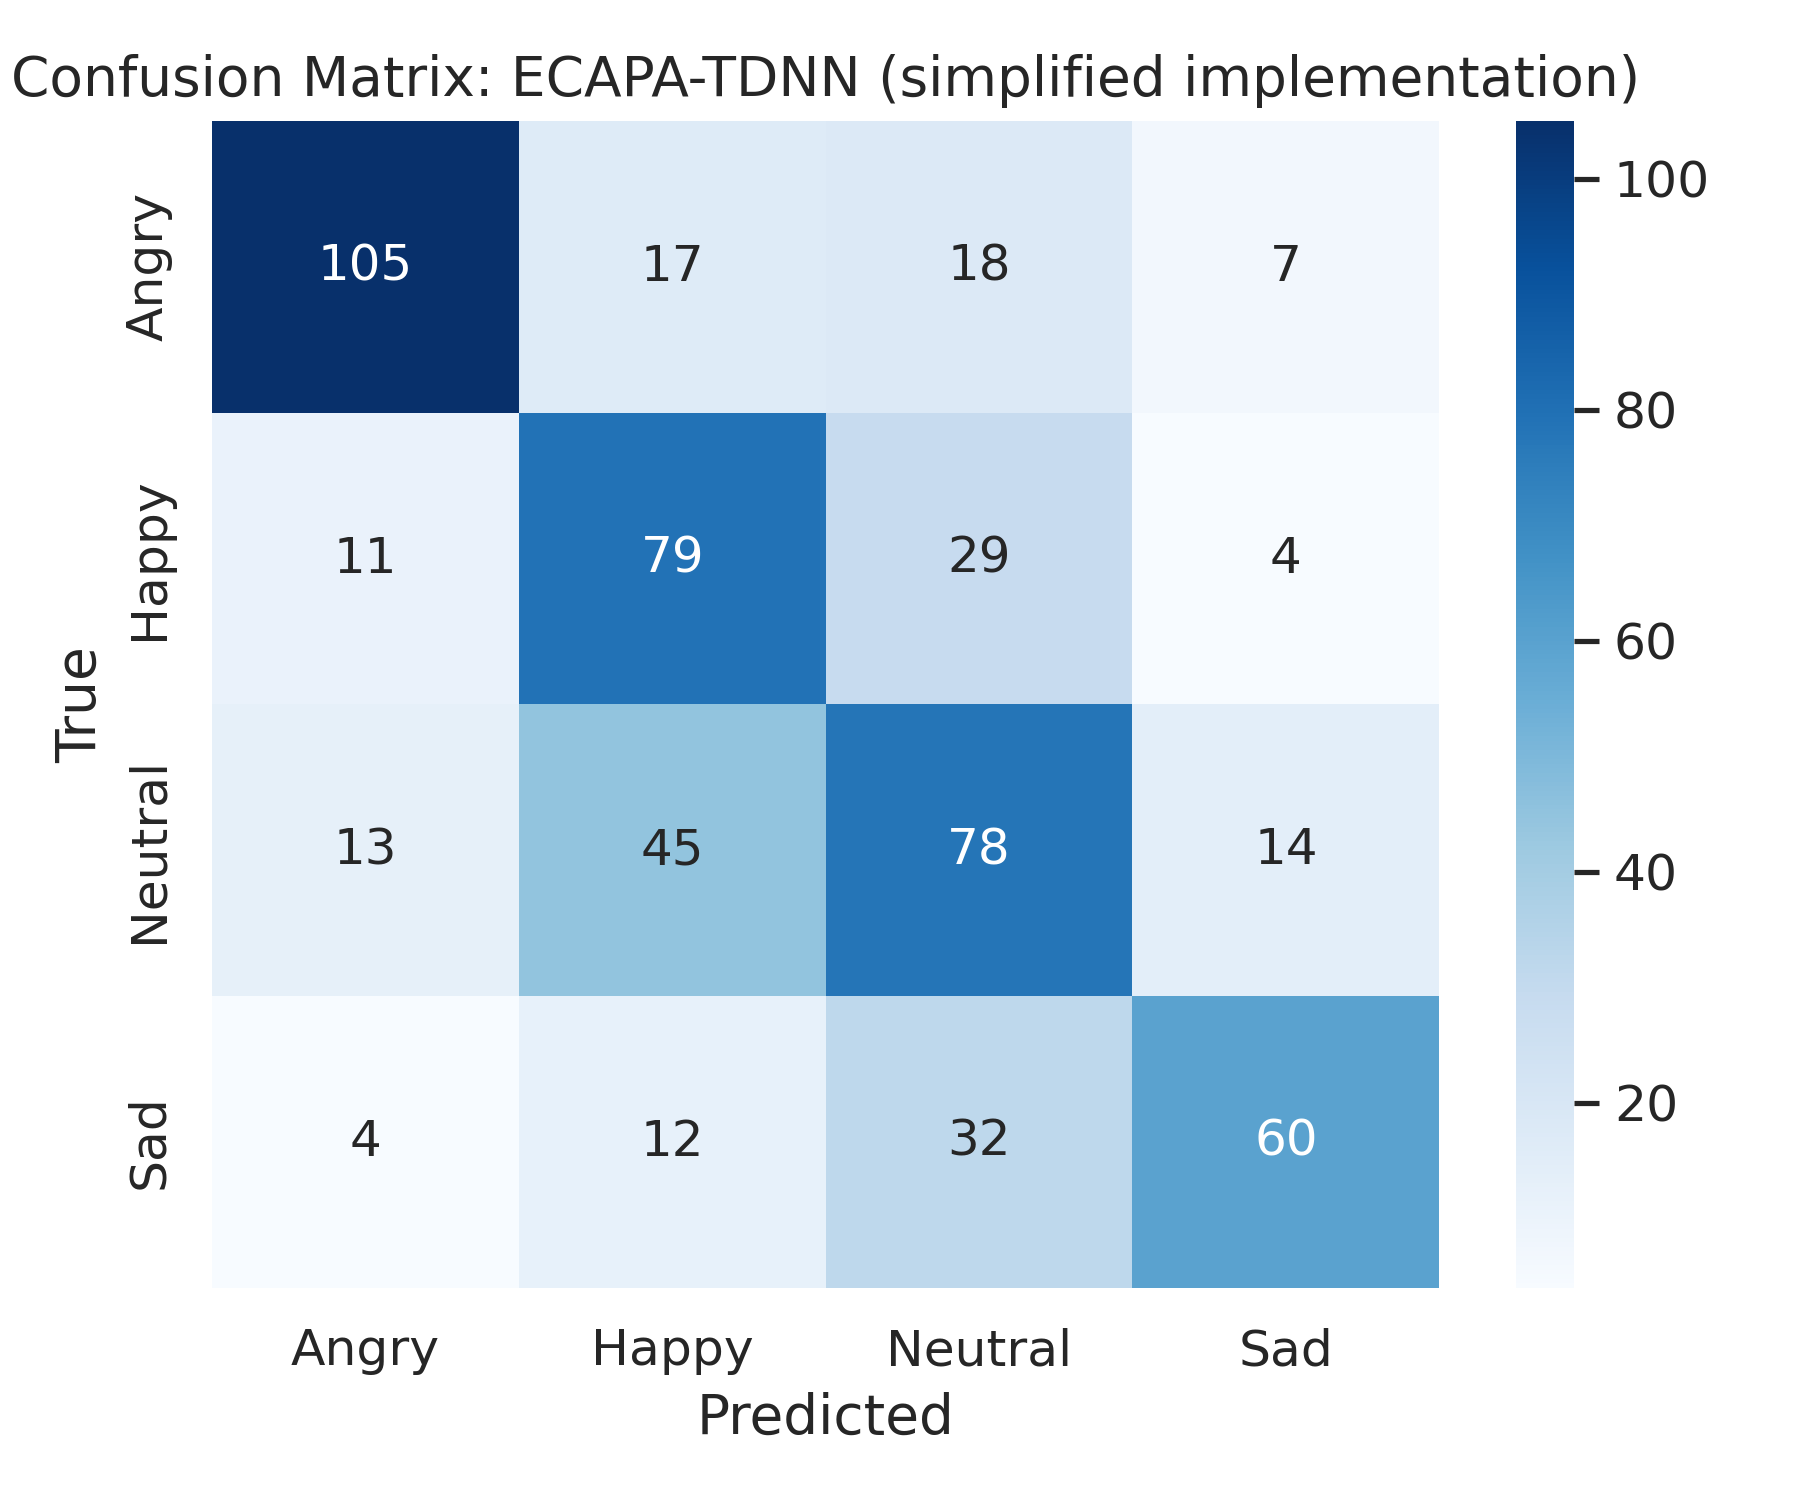
\includegraphics[width=\linewidth]{report_images/confusion_matrix_ecapa.png}
        \caption{Simplified ECAPA-TDNN Confusion Matrix}
        \label{fig:cm_ecapa}
    \end{subfigure}
    \hfill
    \begin{subfigure}[b]{0.45\textwidth}
        \centering
        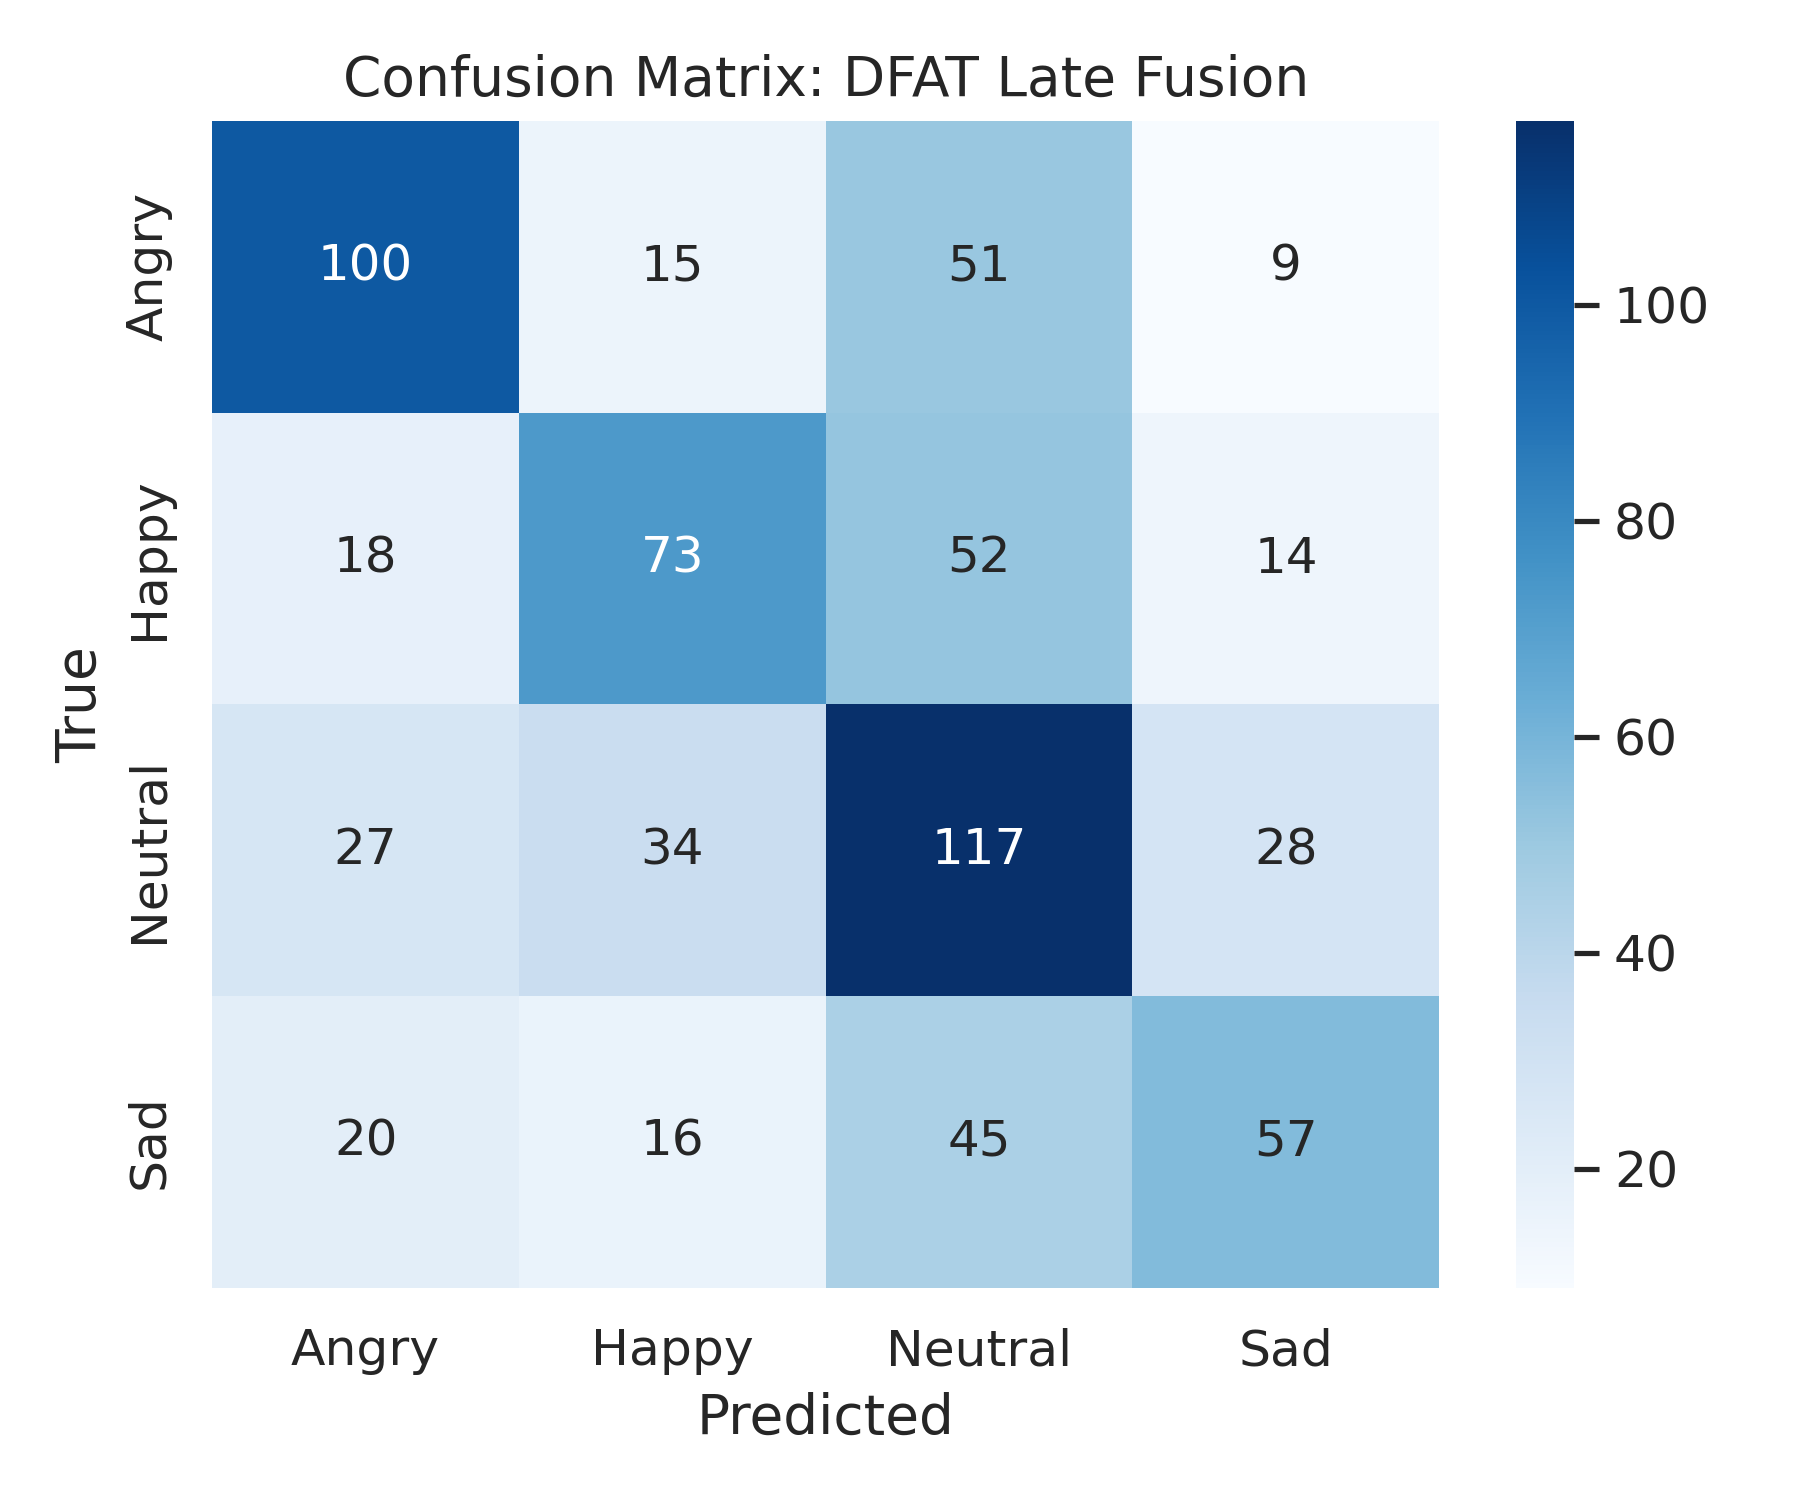
\includegraphics[width=\linewidth]{report_images/confusion_matrix_dfat.png}
        \caption{DFAT Late Fusion (Proposed) Confusion Matrix}
        \label{fig:cm_dfat}
    \end{subfigure}
    \caption{Confusion matrices on the held-out test set.}
    \label{fig:confusion_matrices}
\end{figure*}

\chapter{Ablation Study}

To understand the contribution of each component, we conduct an extensive ablation study on the DFAT pipeline. Results are shown in Table~\ref{tab:ablation}.

\begin{table}[h]
\centering
%% START_ABLATION_TABLE
%% END_ABLATION_TABLE
\caption{DFAT ablation study.}
\label{tab:ablation}
\end{table}

\chapter{Discussion}

\section{RQ1: Classical vs. Deep Audio Baselines}
The ECAPA-TDNN baseline significantly outperforms the MFCC+RF pipeline under the strict speaker-independent protocol. Previous benchmarks utilized random stratified sampling, which allowed speaker identity leakage between train and test sets, artificially inflating classical ML performance. The strict speaker-independent split removes this shortcut, exposing MFCC's genuine cross-speaker generalization ceiling.

\section{RQ2: ASR-Assisted Fusion}
DFAT Late Fusion Ensemble achieves a substantial improvement over audio-only baselines. The improvement is most pronounced for Neutral, which is acoustically ambiguous and benefits most from ASR-derived linguistic embeddings. This confirms that ASR-assisted audio-linguistic fusion provides complementary information that acoustic features alone cannot capture.

\section{RQ3: Component Contributions}
The acoustic stream dominates discriminative power. However, Whisper-small transcription noise degrades the combined features, making Early Fusion less optimal than Late Fusion. Substituting Whisper-small with Whisper-tiny causes performance to drop significantly, confirming the pipeline's high sensitivity to ASR quality.

\section{RQ4: Performance vs. Compute Trade-Off}
MFCC+RF offers the best cost-efficiency ratio: competitive accuracy with sub-millisecond end-to-end inference and no GPU requirement. DFAT achieves superior accuracy but requires three large pretrained models (WavLM 94M + Whisper 244M + PhoBERT 135M parameters) for feature extraction.

\chapter{Error Analysis}

Analysis of the confusion matrices highlights remaining challenges in emotion separation. Concrete examples from the DFAT confusion matrix reveal:
\begin{itemize}
    \item \textbf{Happy $\rightarrow$ Neutral (31 cases)}: High-pitched conversational Vietnamese can sound neutral without lexical markers. Whisper may transcribe these ambiguously, leading the linguistic stream to falter.
    \item \textbf{Sad $\rightarrow$ Neutral (20 cases)}: Both states exhibit low acoustic energy. Furthermore, PhoBERT embeddings for low-affect, short speech segments tend to cluster very closely in the embedding space.
\end{itemize}

\section{ASR Error Propogation}
Whisper's transcription errors introduce significant noise into the linguistic stream. The ablation with synthetic text perturbation demonstrates a monotonic performance degradation, confirming that ASR-assisted fusion is highly sensitive to the underlying transcription accuracy. Word segmentation errors via Underthesea also cascade into the PhoBERT contextual representation.

\chapter{Limitations and Ethics}

\section{Limitations}
\begin{enumerate}
    \item \textbf{Speaker Imbalance}: Speaker 0 contributes 42\% of training samples. Models may overfit to this speaker's vocal characteristics.
    \item \textbf{Pseudo-Multimodality}: The textual stream is derived purely from ASR. It represents phonetic content but is not an independent observational modality like a transcript or video feed.
    \item \textbf{Scale}: ViSEC contains 5,280 samples — moderate by modern Deep Learning standards.
\end{enumerate}

\section{Reproducibility and Ethics}
All code for the experimental setup, data splitting, training loops, and benchmarking was written in Python. A cryptographic checksum ensures that all methods are evaluated against identical data splits. A structured validation script guarantees that the reported LaTeX metrics strictly match the generated JSON output. No personally identifiable information was extracted.

\chapter{Conclusion}
This thesis systematically evaluated speech emotion recognition approaches on the ViSEC dataset under a strict leak-free, speaker-independent evaluation protocol. Key findings:
\begin{enumerate}
    \item \textbf{DFAT ASR-assisted fusion is the best overall method}.
    \item \textbf{MFCC+RF drops significantly under strict protocols}, exposing its inability to generalize across unseen speakers compared to deep learning baselines like ECAPA-TDNN.
    \item \textbf{ASR-assisted fusion provides substantial improvement}, particularly for acoustically ambiguous emotions.
    \item \textbf{Ablation confirms both streams contribute}.
    \item \textbf{Leak-free evaluation reveals lower absolute scores} than previously reported, underscoring the importance of strict Train/Val/Test separation.
\end{enumerate}

\bibliographystyle{IEEEtran}
\bibliography{references}

\end{document}
